\documentclass[a4paper]{article}
\usepackage[utf8]{inputenc}

%% %%%%%%%%%%%%%%%%%%%%%%%%%%%%%%%%%%%%%%%%%%%%%%%%%%%%%%%%%%%%%%%%%%%%%%%%%%%%%
%% %%%%%%% %% %% %  %                                      %  % %% %% %%%%%%%%%%
%%%%% %% %  %                    MES COMMANDES                     %  % %% %%%%%
%%%%%%%%%% %% %% %  %                                      %  % %% %% %%%%%%% %%
%%%%%%%%%%%%%%%%%%%%%%%%%%%%%%%%%%%%%%%%%%%%%%%%%%%%%%%%%%%%%%%%%%%%%%%%%%%%% %%

\newcommand{\zzpackages}[1][french]{
  \usepackage[utf8]{inputenc}
  \usepackage[T1]{fontenc}
  \usepackage[#1]{babel}

  \usepackage{amsthm}
  \usepackage{amsmath}
  \usepackage{amsfonts}
  \usepackage{amssymb}

  \usepackage{xcolor}
  \usepackage{xstring}	%\ifstreqcase
}

%% %%%%%%%%%%%%%%%%%%%%%%%%%%%%%%%%%%%%%%%%%%%%%%%%%%%%%%%%%%%%%%%%%%%%%%%%%%%%%
%                              TESTS / FOR / ...                               %
%%%%%%%%%%%%%%%%%%%%%%%%%%%%%%%%%%%%%%%%%%%%%%%%%%%%%%%%%%%%%%%%%%%%%%%%%%%%% %%

% 
\def\defactive#1#2{
  \catcode`#1=13
  \begingroup
  \lcode`~=`#1
  \lowercase{\endgroup\def~}{#2}
}

\def\zifempty#1#2#3{\def\foo{#1}\ifx\foo\empty\relax#2\else#3\fi}

%% %%%%%%%%%%%%%%%%%%%%%%%%%%%%%%%%%%%%%%%%%%%%%%%%%%%%%%%%%%%%%%%%%%%%%%%%%%%%%
%                           MARGES / HYPERREF / ...                            %
%%%%%%%%%%%%%%%%%%%%%%%%%%%%%%%%%%%%%%%%%%%%%%%%%%%%%%%%%%%%%%%%%%%%%%%%%%%%% %%

\makeatletter
\gdef\@subtitle{}
\def\subtitle#1{\gdef\@subtitle{#1}}

\def\zztitre{
\begingroup\centering
{\bfseries \huge \@title}\par\vspace{.3cm}
\ifx\@subtitle\empty\else{\bfseries \Large \@subtitle}\par\vspace{.5cm}\fi
\Large \@author\par\vspace{.1cm}
\@date\zal\vspace{.3cm}\zal
\zligne\endgroup
}

\makeatother


\newcommand{\zzhyperref}{
\usepackage{hyperref}
\hypersetup{ colorlinks=true, linkcolor=blue!30!black,
citecolor=green!30!black, filecolor=magenta!30!black,
urlcolor=cyan!30!black }
}

\newcommand{\zzmarges}{
  \setlength{\textheight}{620pt}
  \addtolength{\textwidth}{2cm}
  \addtolength{\hoffset}{-1cm}
  \addtolength{\voffset}{-1cm}
  \addtolength{\marginparwidth}{0cm}
  \addtolength{\textheight}{1cm}
} 

\makeatletter
\newcommand{\zzheader}[6]{
\def\@oddhead{\vbox to 0pt{\vss\hspace{0pt} #1\hfill #2\hfill #3\kern4pt\par\kern5pt\hrule height.5pt}}
\def\@oddfoot{\vbox to 0pt{\hrule height.5pt\kern5pt\hbox to \linewidth{\kern4pt {#4}\hss {#5}\hss {#6}\kern4pt}\vss}}}
\makeatother

%%%%%%%%%%%%%%%%%%%%%%%%%%%%%%%%%%%%%%%%%%%%%%%%%%%%%%%%%%%%%%%%%%%%%%%%%%%%%%%%

\newcommand{\zligne}[1][]{
\par\zifempty{#1}%
{\hbox to \linewidth{\leaders\hrule height3pt depth-2.5pt\hfill}}%
{\hbox to \linewidth{\leaders\hrule height3pt depth-2.5pt\hfill\kern.8em #1\kern.8em\leaders\hrule height3pt depth-2.5pt\hfill}}\par
}

%%%%%%%%%%%%%%%%%%%%%%%%%%%%%%%%%%%%%%%%%%%%%%%%%%%%%%%%%%%%%%%%%%%%%%%%%%%%%%%%

\newcommand{\zal}{\par}
\newcommand{\znl}{\zal ~\zal}
\newcommand{\zguill}[2][]{«\,#2\,»}

%% %%%%%%%%%%%%%%%%%%%%%%%%%%%%%%%%%%%%%%%%%%%%%%%%%%%%%%%%%%%%%%%%%%%%%%%%%%%%%
%                             COMMANDES PRATIQUES                              %
%%%%%%%%%%%%%%%%%%%%%%%%%%%%%%%%%%%%%%%%%%%%%%%%%%%%%%%%%%%%%%%%%%%%%%%%%%%%% %%

%% ------- -- -- -  -                                      -  - -- -- --------%%
%---- -- -  -                          ZP                          -  - -- ----%
%%-------- -- -- -  -                                      -  - -- -- ------- %%
\makeatletter
\def\z@first#1#2{#1}
\def\z@second#1#2{#2}
\def\z@zp@selectchar#1#2{
  \IfStrEqCase{#2}{%
    {p}{#1{(}{)}}%
    {c}{#1{[}{]}}%
    {a}{#1{\{}{\}}}%
    {C}{#1{]}{[}}%
    {b}{#1{|}{|}}%
    {n}{#1{\|}{\|}}%
    {i}{#1{[}{]}\!#1{[}{]}}%
    {t}{#1{<}{>}}%
    {v}{#1{.}{.}}%
    {A}{#1{\}}{\{}}%
    {P}{#1{)}{(}}%
    {I}{#1{]}{[}\!#1{]}{[}}%
    {T}{#1{>}{<}}%
  }[#1{(}{)}]%
}

\def\z@zp#1#2\fin#3{
  \z@zp@selectchar{\left\z@first}{#1}#3
  \zifempty{#2}%
        {\z@zp@selectchar{\right\z@second}{#1}}%
        {\z@zp@selectchar{\right\z@second}{#2}}%
}
\newcommand{\zp}[2][]{\zifempty{#1}{\left(#2\right)}{\z@zp#1\fin{#2}}}

\newcommand{\zpbig}[1]{\ifcase#1\relax\vrule width0pt height0pt\or\vrule width0pt height9pt\or\vrule width0pt height10pt\or\vrule width0pt height13pt\else\vrule width0pt height16pt\fi}

%% ------- -- -- -  -                                      -  - -- -- --------%%
%---- -- -  -                   Itemize et autre                   -  - -- ----%
%%-------- -- -- -  -                                      -  - -- -- ------- %%

\newcommand{\zitemize}[1]{
\vspace{-\topsep}\begin{itemize}\setlength\itemsep{0pt plus 1pt}\setlength\parskip{0cm}#1\end{itemize}\vspace{-\topsep}}


%% ------- -- -- -  -                                      -  - -- -- --------%%
%---- -- -  -                        AUTRES                        -  - -- ----%
%%-------- -- -- -  -                                      -  - -- -- ------- %%

\newcommand{\zR}{\mathbb{R}}

\newcommand{\zsum}[2][0pt]{\sum_{\hbox to #1{\hss$\scriptstyle#2$\hss}}}
\newcommand{\zprod}[2][0pt]{\prod_{\hbox to #1{\hss$\scriptstyle#2$\hss}}}

\newcommand{\zseq}[1][=]{\hspace{2pt}\raise .5pt\hbox{\scalebox{.8}{#1}}\hspace{2pt}}

\newcommand{\zop}[2]{\mathrm{#1}\zp{#2}}

\newcommand{\zi}{\mathrm{i}}

\newcommand{\zexp}[1]{\mathrm{e}^{#1}}

\newcommand{\zmatrix}[2]{\left(\begin{array}{#1}#2\end{array}\right)}

\newcommand{\zindic}[1]{%
\hbox to 5.3pt{1\hss l}\hskip -2.5pt\left\{#1\right\}%
}

\newcommand{\zesp}[2][]{%              esperance
\mathbb{E}_{#1}\hskip -3pt\left[\zpbig1\,#2\,\right]%
}

\newcommand{\zprob}[2][]{%             proba
\mathbb{P}_{#1}\hskip -3pt\left(\zpbig1\,#2\,\right)%
}

% Symbole d'indépendance de variable aléatoire
\newcommand{\zindep}{\protect\mathpalette{\protect\z@ind}{\perp}}
\def\z@ind#1#2{\mathrel{\rlap{$#1#2$}\mkern6mu{#1#2}}}


\newcommand{\zdx}[1]{\mathrm{d}#1}

\newcommand{\zderiv}[2]{\frac{\partial #1}{\partial #2}}


\newcommand{\ztr}[2][]{\zifempty{#1}{#2}{\left(#2\right)}^{\hspace{-1pt}\mathsf{T}}\hspace{-1pt}}
\def\zpreind#1#2{ \raise-.35ex\hbox{\scriptsize$#1$}#2}
\def\zpreexp#1#2{ \raise.85ex\hbox{\scriptsize$#1$}#2}

%% %%%%%%%%%%%%%%%%%%%%%%%%%%%%%%%%%%%%%%%%%%%%%%%%%%%%%%%%%%%%%%%%%%%%%%%%%%%%%
%                                 ALGORITHMES                                  %
%%%%%%%%%%%%%%%%%%%%%%%%%%%%%%%%%%%%%%%%%%%%%%%%%%%%%%%%%%%%%%%%%%%%%%%%%%%%% %%

\newcount\z@algo@count
\newdimen\z@algo@indent
\begingroup
  \catcode`\^^M=13             %
  \catcode`\^^I=13             %
  \gdef\z@algo{                %
  \z@algo@count=1
    \begingroup                %
    \catcode`\^^M=13           %
    \def^^M{\leavevmode\par \advance\z@algo@count by 1\z@algo@indent=0pt}%
    \catcode`\^^I=13           %
    \def^^I{\advance\z@algo@indent by 1em}         %
    \everypar{                 %
      \hbox to 0cm{\hss\textcolor{black!30}{\the\z@algo@count~:}}~\kern\z@algo@indent}  %
                               %
    \tt                        %
  }

\endgroup

\newenvironment{zalgo}{\z@algo}{\endgroup}


\makeatother



%% %%%%%%%%%%%%%%%%%%%%%%%%%%%%%%%%%%%%%%%%%%%%%%%%%%%%%%%%%%%%%%%%%%%%%%%%%%%%%
%                                    AUTRE                                     %
%%%%%%%%%%%%%%%%%%%%%%%%%%%%%%%%%%%%%%%%%%%%%%%%%%%%%%%%%%%%%%%%%%%%%%%%%%%%% %%

% epaisseur trait / marge / texte

\def\zfbox#1#2#3{
  \hbox{\vrule width #1
    \vtop{
      \vbox{
        \hrule height #1
        \kern #2
        \hbox{\kern #2 #3\kern #2}
      }%
      \kern #2%
      \hrule height #1
    }%
    \vrule width #1%
  }%
}

%% \begin{mygraph}{xmin=0, xmax=1, %
%%                ymin=0, ymax=1, %
%%                sizex=2.5, sizey=2.5}%
%%                {nomx=Axe X, nomy=Axe Y}%
%%                {0,.5,1}{0,0.25,...,1.05}

%% \graduationX[dashed, blue]{ .78 / $\frac{\pi}{4}$ }{ PARAMETRE TEXT }

%% \begin{mylegend}{x=0.3, y=.9, n=2, t=2.1, scale=.5}
%%   \newlegend{blue}{Courbe 1}
%%   \newlegend{red}{Courbe 2}
%% \end{mylegend}

%% \fillbetweencurve[opacity=.2, blue]{ COURBE 1 }{ COURBE 2 }

%% \end{mygraph}


\usepackage{tikz}



\pgfkeys{
%
 /mygraph/.is family, /mygraph,
 xmin/.estore in = \xn,
 xmax/.estore in = \xm,
 ymin/.estore in = \yn,
 ymax/.estore in = \ym,
 sizex/.estore in = \xx,
 sizey/.estore in = \yy,
 %
/mygraphb/.is family, /mygraphb,
 nomx/.estore in = \axex,
 nomy/.estore in = \axey,
%
/mygraphc/.is family, /mygraphc,
 gradsize/.estore in = \gradsize,
 gradsize/.default = 0.1,
 nomydist/.estore in = \axeyd,
 nomydist/.default = 0.8cm,
 gradsize, nomydist,                 % NE PAS OUBLIER
%
/myleg/.is family, /myleg,
 x/.estore in = \legendx,
 y/.estore in = \legendy,
 n/.estore in = \legendn,
 t/.estore in = \legendt,
 scale/.estore in = \legends,
 scale/.default = 1,
 scale,
%
/mylego/.is family, /mylego,
size/.estore in = \legendwidth,
size/.default = 0.4,
size                                  % NE PAS OUBLIER
}


%%%%%%%%%%%%%%%%%%%%%%%%%%%%%%%%%%%%%%%%%%%%%%%%%%%%%%%%%%%%%%%%%%%%%%%%%%%%%%%%
%                                                                              %
%%%%%%%%%%%%%%%%%%%%%%%%%%%%%%%%%%%%%%%%%%%%%%%%%%%%%%%%%%%%%%%%%%%%%%%%%%%%%%%%

\newenvironment{mygraph}[5][]{%
\pgfkeys{/mygraph, #2}
\pgfkeys{/mygraphb, #3}
\pgfkeys{/mygraphc, #1}
  \pgfmathsetmacro\dum{\yy/(\ym-\yn)}
  \pgfmathsetmacro\dumm{\xx/(\xm-\xn)}
\begin{tikzpicture}[yscale=\dum, xscale=\dumm,font=\sffamily]
  \pgfmathsetmacro\gradx{\gradsize / \dum}
  \pgfmathsetmacro\grady{\gradsize / \dumm}

  \foreach \x in {#4}{
    \draw[very thin, color=black, dotted] (\x,\yn) -- (\x,\ym);
    \draw (\x,\yn+\gradx) -- (\x,\yn)
          node[font=\tiny, anchor=north] {\pgfmathprintnumber{\x}};
  };
  \foreach \y in {#5}{
    \draw[very thin, color=black, dotted] (\xn,\y) -- (\xm,\y); 
    \draw (\xn+\grady,\y) -- (\xn,\y)
          node[font=\tiny, anchor=east] {\pgfmathprintnumber{\y}};
  };
  \draw (\xn,\yn) -- node[font=\scriptsize, below=0.3cm] {\axex} (\xm,\yn);
  \draw (\xn,\yn) -- node[font=\scriptsize, rotate=90, above=\axeyd, anchor=mid] {\axey} (\xn,\ym);
  \draw (\xn,\ym) -- (\xm,\ym);
  \draw (\xm,\yn) -- (\xm,\ym);

  \begin{scope}
    \clip (\xn,\yn) rectangle (\xm,\ym);
    %% \draw[dashed] (\xn, 0) -- (\xm, 0);
    %% \draw[dashed] (0, \yn) -- (0, \ym);
}{
  \end{scope}
\end{tikzpicture}
}

%%%%%%%%%%%%%%%%%%%%%%%%%%%%%%%%%%%%%%%%%%%%%%%%%%%%%%%%%%%%%%%%%%%%%%%%%%%%%%%%

\newenvironment{mylegend}[2][]{
\pgfkeys{/myleg, #2}
\pgfkeys{/mylego, #1}
\begin{scope}[shift={(\legendx,\legendy)}, scale=\legends]
\pgfmathsetmacro\legendwidth{\legendwidth * (\xm-\xn) / \xx }
\pgfmathsetmacro\dum{ (0.125 * (\ym-\yn) / \yy) }
\pgfmathsetmacro\dumm{ - (0.125 * (\xm-\xn) / \xx) }
\pgfmathsetmacro\legendy{ 0 }
\coordinate (dum) at (\dumm,\dum);
\pgfmathsetmacro\dum{ - (\legendn-0.4)*(0.25 * (\ym-\yn) / \yy) }
\coordinate (dumm) at (\dumm,\dum);
\pgfmathsetmacro\dumm{\dumm + (\legendt * (\xm-\xn) / \xx) }
\draw[fill=white, opacity=.8] (dum) -- (dumm) -| (\dumm,\dum) |- (dum);
}{
\end{scope}
%% \pgfmathsetmacro\legendyi{\legendyi + (0.125 * (\ym-\yn) / \yy)  }
%% \pgfmathsetmacro\legendy{\legendy + (0.1 * (\ym-\yn) / \yy)  }
%% \pgfmathsetmacro\legendx{\legendx - (0.125 * (\xm-\xn) / \xx)  }
%% \draw[] (\legendx,\legendyi) -- (\legendx,\legendy) %
%%                              -| (\legendx + 1,\legendy)
%%                              |- (\legendx,\legendyi);
}

\newcommand{\newlegend}[2]{
\draw[font=\scriptsize, #1] (0,\legendy) -- (\legendwidth,\legendy)	node[right,scale=\legends]{#2};
\pgfmathsetmacro\legendy{\legendy - (0.25 * (\ym-\yn) / \yy)  }
}

%%%%%%%%%%%%%%%%%%%%%%%%%%%%%%%%%%%%%%%%%%%%%%%%%%%%%%%%%%%%%%%%%%%%%%%%%%%%%%%%

\newenvironment{outofbox}{%
  \end{scope}%
}{%
  \begin{scope}%
    \clip (\xn,\yn) rectangle (\xm,\ym);%
}

%%%%%%%%%%%%%%%%%%%%%%%%%%%%%%%%%%%%%%%%%%%%%%%%%%%%%%%%%%%%%%%%%%%%%%%%%%%%%%%%

\newcommand{\fillbetweencurve}[3][]{
\begin{scope}
\clip (\xn,\yn) -- #2 -- (\xm,\yn) -- cycle;
\fill[#1] (\xn,\ym) -- #3 -- (\xm,\ym) -- cycle;
\end{scope}
}

%%%%%%%%%%%%%%%%%%%%%%%%%%%%%%%%%%%%%%%%%%%%%%%%%%%%%%%%%%%%%%%%%%%%%%%%%%%%%%%%

\newcommand{\graduationX}[3][very thin, color=black, dotted]{
\end{scope}
  \foreach \x/\t in {#2}{
    \draw[#1] (\x,\yn) -- (\x,\ym);
    \draw (\x,\yn+\gradx) -- (\x,\yn)
          node[font=\tiny, anchor=north, #3] {\t};
  };
\begin{scope}%
\clip (\xn,\yn) rectangle (\xm,\ym);%
}

%%%%%%%%%%%%%%%%%%%%%%%%%%%%%%%%%%%%%%%%%%%%%%%%%%%%%%%%%%%%%%%%%%%%%%%%%%%%%%%%

\newcommand{\graduationY}[3][very thin, color=black, dotted]{
\end{scope}
  \foreach \y/\t in {#2}{
    \draw[#1] (\xn,\y) -- (\xm,\y);
    \draw (\xn+\grady,\y) -- (\xn,\y)
          node[anchor=east, font=\tiny, shift={(-0*\grady,0)}, #3] {\t};
  };
\begin{scope}%
\clip (\xn,\yn) rectangle (\xm,\ym);%
}


\zzpackages[english]
\zzhyperref
\zzmarges

\zzheader{PGM Project}{}{\today}{De Lara, Tilquin, Vidal}{}{\arabic{page}/\pageref{lastpage}}

%% %%%%%%%%%%%%%%%%%%%%%%%%%%%%%%%%%%%%%%%%%%%%%%%%%%%%%%%%%%%%%%%%%%%%%%%%%%%%%
%                                MACRO LOCALES                                 %
%%%%%%%%%%%%%%%%%%%%%%%%%%%%%%%%%%%%%%%%%%%%%%%%%%%%%%%%%%%%%%%%%%%%%%%%%%%%% %%

% Divergence de Kullback-Leibler
\newcommand{\Kl}[3][]{\mathrm K_{#1}\!\zp{#2\:\|\:#3}}
\newcommand{\zZ}[2]{\mathrm #1\!\zp{#2}}
\newcommand{\zD}{\mathcal}
\newcommand{\Ng}[2]{\mathcal{N}\zp{#1,\:#2}}

\tikzset{
  zplot/.style={opacity=.8}
}

%% %%%%%%%%%%%%%%%%%%%%%%%%%%%%%%%%%%%%%%%%%%%%%%%%%%%%%%%%%%%%%%%%%%%%%%%%%%%%%
%                                DEBUT DOCUMENT                                %
%%%%%%%%%%%%%%%%%%%%%%%%%%%%%%%%%%%%%%%%%%%%%%%%%%%%%%%%%%%%%%%%%%%%%%%%%%%%% %%

\begin{document} 

\def\foo#1#2{\vbox{\hbox to 2cm{\hss\scshape #1\hss}\hbox to 2cm{\hss\footnotesize#2\hss}}\hss}

\begingroup\centering
{\bfseries \huge Independent Component Analysis}\par\vspace{.3cm}
{\bfseries \Large PGM Project}\par\vspace{.7cm}
\hbox to \textwidth{\hss
\foo{Nathan de Lara}{École polytechnique}
\foo{Florian Tilquin}{ENS Cachan}
\foo{Vincent Vidal}{ENS Ulm}
}\par\vspace{.8cm}
\today\zal\vspace{.3cm}\zal
\zligne\endgroup

\tableofcontents

\vspace{1cm}\zligne


\begin{center}\textsc{Abstract}\end{center}
This paper is dedicated to the study of Independent Component Analysis. We intent to implement, apply and compare several algorithms while being presenting some theoretical aspects such as the link between the likelihood maximisation and the mutual information.

%% ------- -- -- -  -                                      -  - -- -- --------%%
%---- -- -  -                     Introduction                     -  - -- ----%
%%-------- -- -- -  -                                      -  - -- -- ------- %%


\section{Problem statement}
\subsection{Introduction}

The general Independent Component Analysis problem can be formalised this way:
Suppose we have some random variables $x\in\zR^p$ which correspond to
a mix of some primitive sources $s\in\zR^n$. The aim is to extract
from $x$ every source $s_i$. To do so, we will suppose here that:
\zitemize{
\item[--] the sources are independents.
\item[--] the mix is linear and instantaneous
\item[--] at most one source has a Gaussian distribution.
}
We define:
\begin{equation}
  x = A s \ \ \mbox{and} \ \ y = W x,
\end{equation}
where $A$ is the mixing matrix, $W$ the separation matrix and $y$ the
estimation of the sources. The goal is then to find a matrix $W$ that
maximise a certain measure of independence of $y$.

As a measure of independence, we consider, for theoretical purpose,
the mutual information:\begin{equation}
  \zZ IY = \int_{\zR^p} P(Y) \log\frac{P(Y)}{\Pi_i P_i(Y_i)} \zdx Y.
\end{equation}
However, as it is too hard to compute, we consider other contrast functions, invariant by permutation, scaling on coordinates and maximal for independent ones.


%% --------- ---- -  -         Information Theory         -  - ---- --------- %%

\subsection{Information Theory}
\label{infth}
Let $X\in\zR^n$ be a random variable, we note $P\zp{X}$ his density and $\Sigma_X$ his covariance matrix.
\znl

In the space of measures, let $\zD G$ be the manifold of Gaussian distributions, $\zD P$ the manifold of ``product'' distributions and $\zD P\wedge\zD G$ the manifold of Gaussian ``product'' distributions. Note that these manifolds are exponential families.

The main advantage of this geometric point of view is that the Kullback-Leibler divergence allows the notion of projection on exponential families. The projection of $P$ on the family $\zD E$ is defined as the vector of $\zD E$ that minimise the divergence to $P$. We write this projection~$P^{\zD E}$.
\znl

Then, we define:

The \textbf{Kullback--Leibler divergence} distribution from $Q$ to $P$:
\begin{equation}
  \Kl PQ = \int_{\zR^n} P(x) \log\frac{P(x)}{Q(x)} \zdx x.
\end{equation}

The \textbf{entropy}:\begin{equation}
  \zZ HP = - \int_{\zR^n} P(x)\log P(x) \zdx x.
\end{equation}

The \textbf{mutual information}:
\begin{equation}
  \zZ IY = \Kl {\zpbig2 P(Y)}{\Pi_i P_i(Y_i)} = \Kl {\zpbig2 P(Y)}{P(Y)^{\zD P}}.
\end{equation}

The \textbf{negentropy}:
\begin{equation}
  \mathrm{G}_n(Y) = \zZ H{\Ng{\zesp Y}{\Sigma_Y}\zpbig2}-\zZ HY= \zZ H{P(Y)^{\zD G}}-\zZ H{P(Y)}.
\end{equation}


The \textbf{non-gaussianity}:
\begin{equation}
  \zZ GY = \Kl{Y}{\Ng{\zesp Y}{\Sigma_Y}\zpbig2} = \Kl {\zpbig2 P(Y)}{P(Y)^{\zD G}}.
\end{equation}

The \textbf{correlation}:
\begin{equation}\begin{array}{rcl}
  \zZ CY &=& \displaystyle\Kl{\Ng{\zesp Y}{\Sigma_Y}\zpbig2}{\Ng{\zesp Y}{\mathrm{Diag}\:\Sigma_Y}}\\
  &=&\Kl{\zpbig2 P(Y)^{\zD G}}{P(Y)^{\zD P\wedge\zD G}}\\
  &=& \displaystyle\frac 12\log\frac{\det\zp{\mathrm{Diag}(\Sigma_Y)}}{\det\zp{\Sigma_Y}}.
\end{array}\end{equation}
\begin{figure}\centering
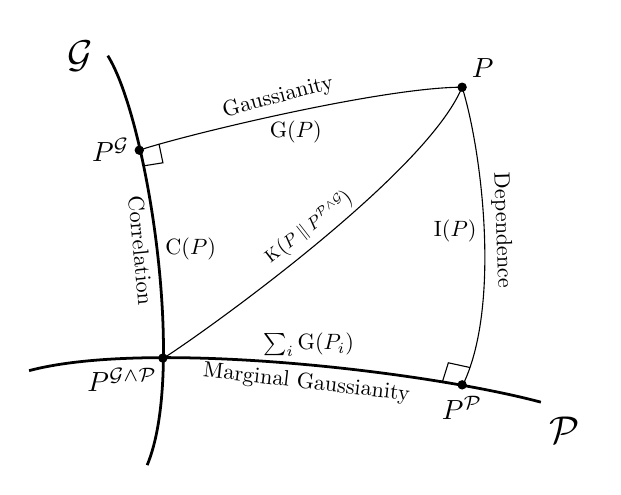
\begin{tikzpicture}[xscale=5, yscale=4, zvar/.style={line width = 1}, zdis/.style={scale=1}, zindic/.style={scale=.8}, zindict/.style={sloped, scale=.8}]
  \draw[zvar](0,-.3) .. controls (.1,0) and (0,.8) .. node[zindict, anchor=north]{Correlation} node[zindic, anchor=west]{$\zZ CP$} (-.1,1) node[anchor=0, scale=1.4]{$\zD G$};
  \draw[zvar](-.3,0) .. controls (0,.1) and (.7,0) .. node[pos=.54, zindict, anchor=north]{Marginal Gaussianity} node[pos=.54, zindic, anchor=south]{$\sum_i\zZ G{P_i}$} (1,-.1) node[anchor=130, scale=1.4]{$\zD P$};
  \draw (.8,.9) node[anchor=south west,zdis]{$P$} .. controls (.6,.9) and (.1,.75) .. node[zindict, anchor=-70]{Gaussianity} node[zindic, anchor=110]{$\zZ GP$} (-.02,.7) node[anchor=east,zdis]{$P^{\zD G}$};
  \draw (-.01,.65) -- (.04,.66) -- (.03,.72);
  \draw (.8,.9) .. controls (.85,.7) and (.9,.2) .. node[zindict, anchor=south]{Dependence} node[zindic, anchor=east]{$\zZ IP$} (.8,-.05) node[anchor=north,zdis]{$P^{\zD P}$};
  \draw (.75,-.035) -- (.765,.025) -- (.82,.01);
  \draw (.8,.9) .. controls (.7,.6) and (.05,.04) .. node[zindic,rotate=38,scale=.8, anchor=south,pos=.45] {$\Kl P{P^{\zD P\wedge\zD G}}$} (.037,.037);
\node[anchor=north east,zdis] at (.05,.04) {$P^{\zD G\wedge \zD P}$};
\foreach \x/\y in{.8/.9,.04/.04,.8/-.045,-.02/.7}{\draw[fill,shift={(\x,\y)}, xscale=.80] (0,0) circle (.013);}
\end{tikzpicture}  
\caption{Representation of a distribution $P$ and the different projections on the exponential families $\zD P$ and $\zD G$. On the paths between the distributions are the quantities associated to the Kullback-Leibler divergence between those distributions.}\label{fig:pythagorean}
\end{figure}

Using the Pythagorean theorem and the two decompositions of $\Kl P{P^{\zD P\wedge\zD G}}$, through $P^{\zD P}$ or $P^{\zD G}$, shown in the Figure \ref{fig:pythagorean}, we can prove that:
\begin{equation}
        \zZ IY + \sum_i\zZ G{Y_i} = \zZ GY + \zZ CY.
\end{equation}
For more information see~\cite{cardoso2003}.

\subsection{ICA and Maximum Likelihood}
As presented in~\cite{hyvarinen2000}, it is possible to consider ICA as a maximum likelihood problem linked to the infomax principle. 
With the previously introduced notations, the log-likelihood is defined as:
\begin{equation}
L = \sum_t \sum_i \log f_i(w_i^Tx(t))+T\log(|det(W)|)
\end{equation}
Where $f_i$ is the density function of $s_i$. The expectation of this likelihood is:
\begin{equation}
\mathbb{E}[L] = \sum_i \mathbb{E}[\log f_i(w_i^Tx(t))]+\log(|det(W)|)
\end{equation}
In the case where $f_i$ is the actual distribution of $w_i^Tx(t)$, the first term becomes $-\sum_i H(w_i^Tx(t))$ which is one of the independence measures listed in~\ref{infth}.

%% ------- -- -- -  -                                      -  - -- -- --------%%
%---- -- -  -                     Algorithmes                      -  - -- ----%
%%-------- -- -- -  -                                      -  - -- -- ------- %%

\section{Algorithms for ICA}
\subsection{Hérault and Jutten (HJ) algorithm}
This method is based on the neural network principle.
We write $W = \zp{I_n+\widetilde W}^{-1}$ and for a pair of given functions $\zp{f,\:g}$, we adapt $\widetilde W$ as follows:\begin{equation}
\widetilde W_{ij} = f(y_i) g(y_j).
\end{equation}

%% --------- ---- -  -            -----------             -  - ---- --------- %%

\subsection{Jade algorithm}
Several methods are based on the cumulants. The goal here is to annul all the cross cumulants of order $4$.
Thus, the idea is to diagonalize the cumulant tensor which is equivalent to minimise the following contrast function:
\begin{equation}
  c\zp{x} = \sum_{i,k,l}\zp[b]{\zop{Cum}{x_i,x_i^*,x_k,x_l}}^2.
\end{equation}

%% --------- ---- -  -            -----------             -  - ---- --------- %%

\subsection{FastICA algorithm}
The FastICA algorithm is based on the information theory. The goal here is to maximise the marginal non-gaussianity on the whitened data, relying on a non linear quadratic function $f$ with the following rule:\begin{equation}
  \widetilde W_{t+1} = \zesp{X.\ztr{f(\ztr{W_t}X)}} - \zesp{f''(\ztr{W_t}X)}W_t,
\end{equation}
with $W_t$ the normalise vector of $\widetilde W_t$. In our experiments, we used $f(x) = \frac{x^4}4$. But it is possible to use $f(x) = \log \cosh x$ or $f(x) = \exp\zp{-\frac{x^2}2}$ as well.

\subsection{Kernel ICA algorithm}
Given a reproducing kernel Hilbert space $\mathcal{F}$, this algorithm seeks to minimize the Kernel Generalized Variance defined as:
\begin{equation}
	\widehat{\delta}_{\mathcal{F}}=-\frac{1}{2}\log \underset{i}{\prod}(1-\rho_i^2)
\end{equation}
where the $\rho_i$ are the kernel canonical correlations between the observations components, obtained with computations over the observations Gram matrices.

%% ------- -- -- -  -                                      -  - -- -- --------%%
%---- -- -  -                      Resultats                       -  - -- ----%
%%-------- -- -- -  -                                      -  - -- -- ------- %%

\section{Results}
\paragraph{Performance measure}
The ``Amari divergence'', equation \ref{eqn:amari}, gives a criterion of proximity between two matrices, to evaluate the performance of an algorithm.
If $U$ and $V$ are two $n$-by-$n$ matrices, the Amari error is defined by:
\begin{equation} \label{eqn:amari}
	d(U,V) = \frac{1}{2n}\sum\limits_{i=1}^n \left(\frac{\sum\limits_{j=1}^n|a_{ij}|}{\max_j |a_{ij}|}-1 \right)+\frac{1}{2n}\sum\limits_{j=1}^n \left(\frac{\sum\limits_{i=1}^n|a_{ij}|}{\max_i |a_{ij}|}-1 \right)
\end{equation}
with $a_{ij} = (UV^{-1})_{ij}$.
This function, which is not an actual distance, has the advantage to be invariant by scaling factors and permutations of the matrices components.

\begin{figure}
\label{distrib}
\centering
\includegraphics[scale=0.9]{graph_distrib.pdf}\\
\caption{Distributions used to test the algorithms.}
\end{figure}

\begin{figure}
\label{distres}
\centering
%\resizebox{\textwidth}{!}{
\input{Tableau_Nathan.txt}
\vspace{3mm}
\input{Tableau2.txt}%}
\caption{\textbf{Left:} Average Amari divergence re-scaled by 100 obtained with the listed algorithms for random mix $m=2$ sources of size $N=250$ sampled with twelve different distributions. \textbf{Right:} Same measure for $m$ sources of size $N$ whose distributions are randomly selected among the twelve. The best results are in bold font. An X is put when a standard desktop computer could not compute the result.}
\end{figure}

\begin{figure}
\label{imres}
\centering
\includegraphics[width=.74\textwidth]{../image_test/unmix4.png}
\caption{Application of JADE algorithm to images separation. The first line presents the original sources, the second one the mix and the last one the estimations.}
\end{figure}

%% \begin{figure}\begin{center}
%% \hspace{-.8cm}\begin{mygraph}{xmin=0, xmax=100, %
%%                 ymin=-1, ymax=1, %
%%                 sizex=5, sizey=2.5}%
%%                 {nomx=Sources, nomy=}%
%%                 {0,50,100}{-1,-.5,...,1.05}
%%   \draw[zplot, red] plot file {data/init_sources_2.txt};
%%   \draw[zplot, green!70!black] plot file {data/init_sources_3.txt};
%%   \draw[zplot, blue] plot file {data/init_sources_1.txt};
%% \end{mygraph}\hspace{-1cm}
%% \begin{mygraph}{xmin=0, xmax=100, %
%%                 ymin=-1, ymax=1, %
%%                 sizex=5, sizey=2.5}%
%%                 {nomx=FastICA, nomy=}%
%%                 {0,50,100}{-1,-.5,...,1.05}
%%   \draw[zplot, red] plot file {data/init_fast_1.txt};
%%   \draw[zplot, green!70!black] plot file {data/init_fast_2.txt};
%%   \draw[zplot, blue] plot file {data/init_fast_3.txt};
%% \end{mygraph}

%% \begin{mygraph}{xmin=0, xmax=100, %
%%                 ymin=-1, ymax=1, %
%%                 sizex=5, sizey=2.5}%
%%                 {nomx=HJ, nomy=}%
%%                 {0,50,100}{-1,-.5,...,1.05}
%%   \draw[zplot, red] plot file {data/init_hj_2.txt};
%%   \draw[zplot, green!70!black] plot file {data/init_hj_1.txt};
%%   \draw[zplot, blue] plot file {data/init_hj_3.txt};
%% \end{mygraph}\hspace{-1cm}
%% \begin{mygraph}{xmin=0, xmax=100, %
%%                 ymin=-1, ymax=1, %
%%                 sizex=5, sizey=2.5}%
%%                 {nomx=JADE, nomy=}%
%%                 {0,50,100}{-1,-.5,...,1.05}
%%   \draw[zplot, red] plot file {data/init_jade_3.txt};
%%   \draw[zplot, green!70!black] plot file {data/init_jade_1.txt};
%%   \draw[zplot, blue] plot file {data/init_jade_2.txt};
%% \end{mygraph}
%% \vspace{-.2cm}
%% \caption{Results of the main ICA algorithms on simulated data. Each colour corresponds to a signal. The ``Sources'' graph shows the unmixed signals and the other ones the results of the algorithms. \label{fig:res}}
%% \end{center}\end{figure}


%% %%%%%%%%%%%%%%%%%%%%%%%%%%%%%%%%%%%%%%%%%%%%%%%%%%%%%%%%%%%%%%%%%%%%%%%%%%%%%
%                               FIN DU DOCUMENT                                %
%%%%%%%%%%%%%%%%%%%%%%%%%%%%%%%%%%%%%%%%%%%%%%%%%%%%%%%%%%%%%%%%%%%%%%%%%%%%% %%


\bibliographystyle{alpha}
\bibliography{Biblio}{}
\nocite{*}

\label{lastpage}

\end{document}
